\documentclass[xcolor=pdftex,dvipsnames,table]{beamer}
%
% Choose how your presentation looks.
%
% For more themes, color themes and font themes, see:
% http://deic.uab.es/~iblanes/beamer_gallery/index_by_theme.html
%
\mode<presentation>
{
  \usetheme{default}      % or try Darmstadt, Madrid, Warsaw, ...
  \usecolortheme{default} % or try albatross, beaver, crane, ...
  \usefonttheme{default}  % or try serif, structurebold, ...
  \setbeamertemplate{navigation symbols}{}
  \setbeamertemplate{caption}[numbered]
  \setbeamercolor{framesource}{fg=gray}
  \setbeamerfont{framesource}{size=\tiny}
} 

\usepackage{amsmath}
\usepackage{comment}
\usepackage{geometry}
\usepackage{wrapfig}
\usepackage[english]{babel}
\usepackage[utf8x]{inputenc}
\usepackage[absolute,overlay]{textpos}


\newcommand{\source}[1]{\begin{textblock*}{4cm}(8.7cm,8.6cm)
    \begin{beamercolorbox}[ht=0.5cm,right]{framesource}
        \usebeamerfont{framesource}\usebeamercolor[fg]{framesource} Source: {#1}
    \end{beamercolorbox}
\end{textblock*}}

\title[AI in Chess]{How Computers Play Chess}
\author{Jacky Xu}
\institute{FDM Group}
\date{March 24, 2016}

\begin{document}

\begin{frame}
  \titlepage
\end{frame}

% Uncomment these lines for an automatically generated outline.
%\begin{frame}{Outline}
%  \tableofcontents
%\end{frame}

%%%%%%%%%%%%%%%%%%%%%%%%%%%%%%%%%%%%%%%%%%%%%%%%%%%%%%%%%%%%%%%%%%%%%%%%%%%%%%%%%%%%%%%%%%
\section{Introduction}

\begin{frame}{What is Chess?}
\begin{itemize}
	\item 2-player board game
    \item Originated in around 6 A.D. in India
	\item Turn-based, zero-sum game
	\item Each player has 16 pieces initially, objective is to capture the opponent's king
	\item Games can end in a win, loss, or a draw
\end{itemize}
\end{frame}

\begin{frame}{The Chess Board}
\begin{center}
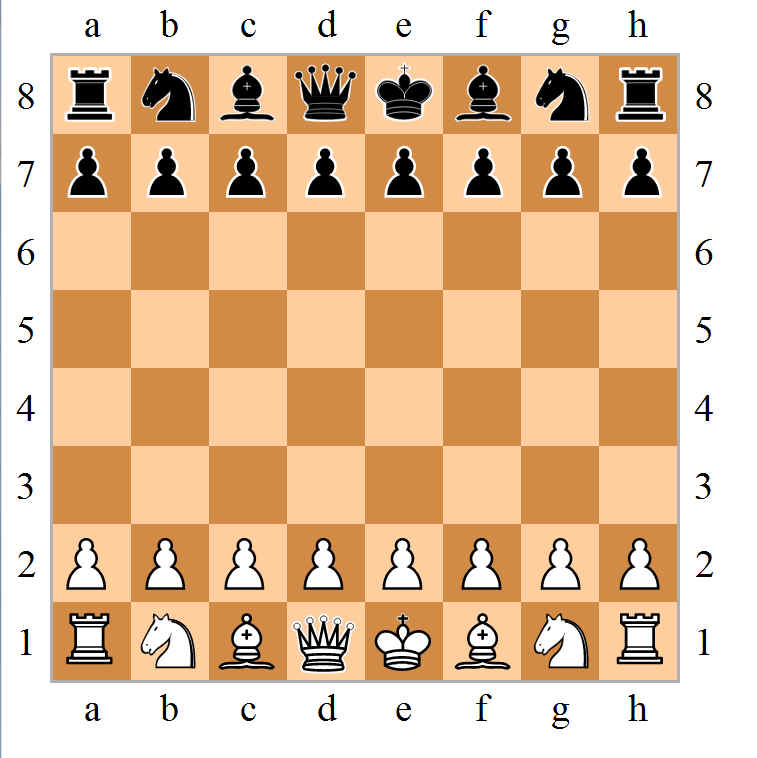
\includegraphics[width=0.7\textwidth,keepaspectratio]{ChessBoard.jpg}
\end{center}
\source{chess-tips.blogspot.com}
\end{frame}

\begin{frame}{History of AI in Chess}
\begin{itemize}
	\item 1769 - "The Turk" by Wolfgang von Kempelen (hoax!)
    \item 1949 - Claude Shannon: "Programming a Computer for Playing Chess"
    \item 1951 - Turing created the first real algorithm for playing Chess: "TUROCHAMP"
    \item 1957 - First programs that can play a full game of chess were made
    \item 1967 - Mac Hack Six becomes the first chess program to win against a human in tournament play ($\sim 1500$ ELO)
    \item 1981 - Cray Blitz wins the Mississippi State Championship with a perfect 5–0 score (first time a computer beats a master in tournament play)
    \item 1997 - Deep Blue defeats Chess champion Kasparov (3.5 - 2.5)
\end{itemize}
\end{frame}

\begin{comment}
HISTORY OF AI IN CHESS
1769 - Hungarian inventor. The Turk defeated Napoleon Bonaparte and Benjamin Franklin. In the early 1820s, it was finally exposed as an elaborate hoax. 
1951 - Since there were no machines that could execute the instructions, Turing had to carry out the calculations by hand and required more than half an hour per move.
1957 - One by American Alex Bernstein and one by Russian programmers
\end{comment}

\begin{frame}{History of AI in Chess}
\begin{center}
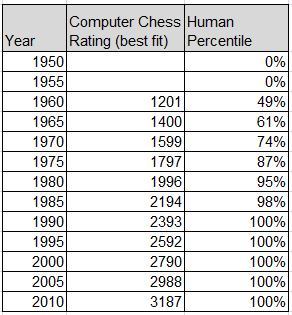
\includegraphics[height=0.6\textheight,keepaspectratio]{chess-ai-rating.png}
\end{center}
\source{chess.com}
\end{frame}

%%%%%%%%%%%%%%%%%%%%%%%%%%%%%%%%%%%%%%%%%%%%%%%%%%%%%%%%%%%%%%%%%%%%%%%%%%%%%%%%%%%%%%%%%%
\section{Components of a Chess Engine}

\begin{frame}{Components of a Chess Engine}
\begin{itemize}
\item Board Representation
\item Move Generator
\item Evaluation
\item Search
\item Opening Books and Tablebases
\end{itemize}
\end{frame}

\begin{frame}{What is a Chess Position?}
\begin{itemize}
\item Position of the pieces
\item Which side to move
\item En-passant square (if any)
\item Castling rights
\item A counter for draw by repetition \& 50-move rule
\end{itemize}
\end{frame}

%%%%%%%%%%%%%%%%%%%%%%%%%%%%%%%%%%%%%%%%%%%%%%%%%%%%%%%%%%%%%%%%%%%%%%%%%%%%%%%%%%%%%%%%%%
\section{Board Representation}

\begin{frame}{Board Representation}
\begin{columns}[c]
\column{1.5in}
\begin{itemize}
\item Piece Centric
	\begin{itemize}
    \item[\textbullet] Piece-Lists
    \item[\textbullet] Piece-Sets
    \item[\textbullet] Bitboards
    \end{itemize}
\vspace{5pt}
\item Square Centric
	\begin{itemize}
    \item[\textbullet] Mailbox
    \item[\textbullet] 8x8 Board
    \item[\textbullet] 10x12 Board
    \item[\textbullet] 0x88
    \item[\textbullet] Vector Attacks
    \end{itemize}
\end{itemize}
\column{2.3in}
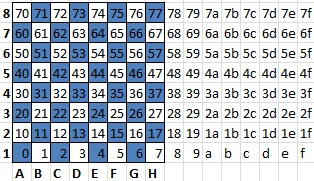
\includegraphics[width=\textwidth,keepaspectratio]{88board.jpg}
\source{chessengine.co.uk}
\end{columns}
\end{frame}

\begin{frame}{Bitboards}
\begin{itemize}
	\item Location of a piece (or pieces) is stored in a 64-bit integer (one bit for every square)
    \item Board is stored using 12 bitboards (one per color per piece-type)
    \item Ideal for x64 architecture (therefore fast!)
    \item Intuitive and easy to apply bitwise operations on multiple bitboards
    \item Used by almost all competitive chess engines today
\end{itemize}
\end{frame}

\begin{frame}{Bitboards (Example)}
\begin{center}
\begin{columns}[c]
\column{0.5\textwidth}
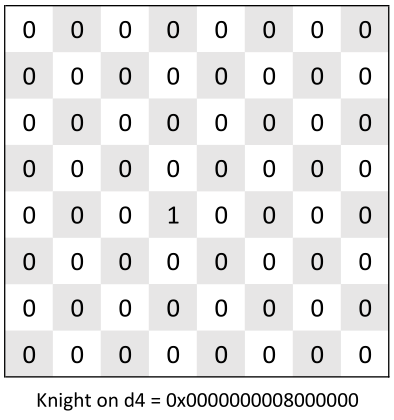
\includegraphics[width=\textwidth,keepaspectratio]{bitboards1.png}
\column{0.5\textwidth}
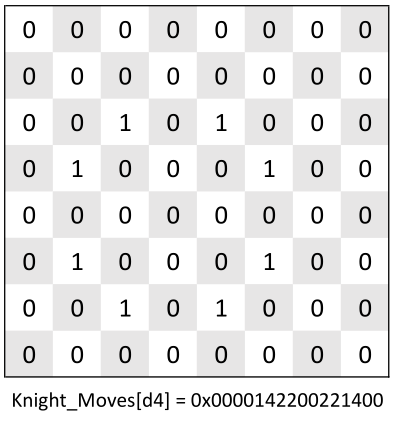
\includegraphics[width=\textwidth,keepaspectratio]{bitboards2.png}
\end{columns}
\end{center}
\end{frame}

%%%%%%%%%%%%%%%%%%%%%%%%%%%%%%%%%%%%%%%%%%%%%%%%%%%%%%%%%%%%%%%%%%%%%%%%%%%%%%%%%%%%%%%%%%
\section{Move Generation}

\begin{frame}{Move Generation}
\begin{itemize}
\item What moves can I make given a particular position?
\item Must ensure moves are legal
	\begin{itemize}
    \item[\textbullet] Destination square cannot be outside board boundaries
    \item[\textbullet] Destination square cannot be occupied by an own piece
    \item[\textbullet] Cannot move into check
    \item[\textbullet] Sliding pieces cannot jump over other pieces
    \item[\textbullet] Must account for special moves (e.g. promotions, castling and en passant)
    \end{itemize}
\item Speed is super important (bitboards are good at this!)
\end{itemize}
\end{frame}

\begin{frame}[fragile]{Move Generation}
\newgeometry{right=-0.5cm}
\begin{wrapfigure}{R}{0.4\textwidth}
	\vspace{-40pt}
	\begin{flushright}
	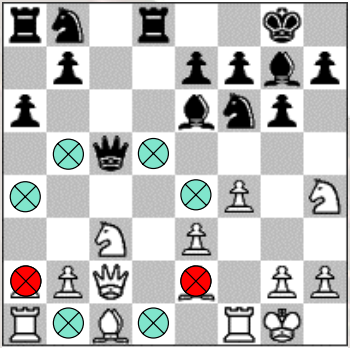
\includegraphics[width=0.4\textwidth,keepaspectratio]{movegen.png}
	\end{flushright}
\end{wrapfigure}
To generate knight moves:
\vspace{20pt}
\small\begin{verbatim}
// 'Knights' is a bitboard of all
// white knights
Knights = B->WhiteKnights;
while (Knights) {
  // Get the first available knight
  from = FirstPiece(Knights);
  // Mask out illegal moves
  to = KnightMoves[from] & ~(B->WhitePieces);     
  // Add potential moves to the global movelist
  AddMovesToList(from,to);
  // Remove this knight from the list
  RemoveFirst(Knights);
}
\end{verbatim}\normalsize
\restoregeometry
\source{cs.bham.ac.uk}
\end{frame}

%%%%%%%%%%%%%%%%%%%%%%%%%%%%%%%%%%%%%%%%%%%%%%%%%%%%%%%%%%%%%%%%%%%%%%%%%%%%%%%%%%%%%%%%%%
\section{Evaluation}

\begin{frame}{Evaluation}
\begin{itemize}
\item Given a position, who has the advantage and by how much?
\item An \underline{evaluation function} looks at the characteristics of a Chess position and returns a score
\item Typically uses a weighted sum model - assign weights to each characteristic and sum the terms up
\end{itemize}
\vspace{5pt}
\begin{equation*}
\begin{split}
score = \hspace{5pt} & weight_{pawn}\cdot(\# White\,Pawns - \# Black\,Pawns) \hspace{5pt} + \\
		& weight_{knight}\cdot(\# White\,Knights - \# Black\,Knights) \hspace{5pt} + \\
        & weight_{bishop}\cdot(\# White\,Bishops - \# Black\,Bishops) \hspace{5pt} + \\
        & weight_{rook}\cdot(\# White\,Rooks - \# Black\,Rooks) \hspace{5pt} + \\
        & weight_{queen}\cdot(\# White\,Queens - \# Black\,Queens) \hspace{5pt}
\end{split}
\end{equation*}
\end{frame}

\begin{frame}{Evaluation}
Other factors to consider:
\begin{itemize}
\item King safety (How many friendly pieces are near my king?)
\item Pawn structure (connected pawns are good, double and isolated pawns are bad)
\item Individual position bonuses for each piece (A knight on the rim is dim)
\item Mobility (How many moves do I have available?)
\item Passed pawns
\item Stage of the game (opening, middle, or endgame?)
\item Many, many, others \dots
\end{itemize}
\end{frame}

%%%%%%%%%%%%%%%%%%%%%%%%%%%%%%%%%%%%%%%%%%%%%%%%%%%%%%%%%%%%%%%%%%%%%%%%%%%%%%%%%%%%%%%%%%
\section{Search}

\begin{frame}{Search}
\begin{itemize}
\item Static evaluation is not enough
\item Must take into account opponent's best move, and our best move in reply, and \dots
\item Keep a game tree, where nodes are positions, and branches are moves
\end{itemize}
\vspace{-10pt}
\begin{center}
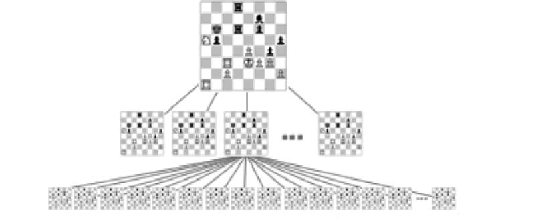
\includegraphics[height=0.4\textheight,keepaspectratio]{gametree2.png}
\end{center}
\source{stanford.edu}
\end{frame}

\begin{frame}{Search: Minimax Algorithm}
Basic idea:
\begin{itemize}
\item MAX-player wants to maximize his score, will always choose the move with the highest score
\item MIN-player wants to minimize her opponent's score, will always choose the move with the lowest score
\end{itemize}
\vspace{5pt}
In the game tree:
\begin{itemize}
\item Eval. of internal nodes = maximum (if MAX-player's turn) or minimum (if MIN-player's turn) evaluation of children nodes
\item Eval. of leaf nodes = calculated from the evaluation function
\item Due to time and space constraints, we stop searching after reaching a certain depth
\end{itemize}
\end{frame}

\begin{frame}{Search: Minimax Algorithm (Example)}
\begin{center}
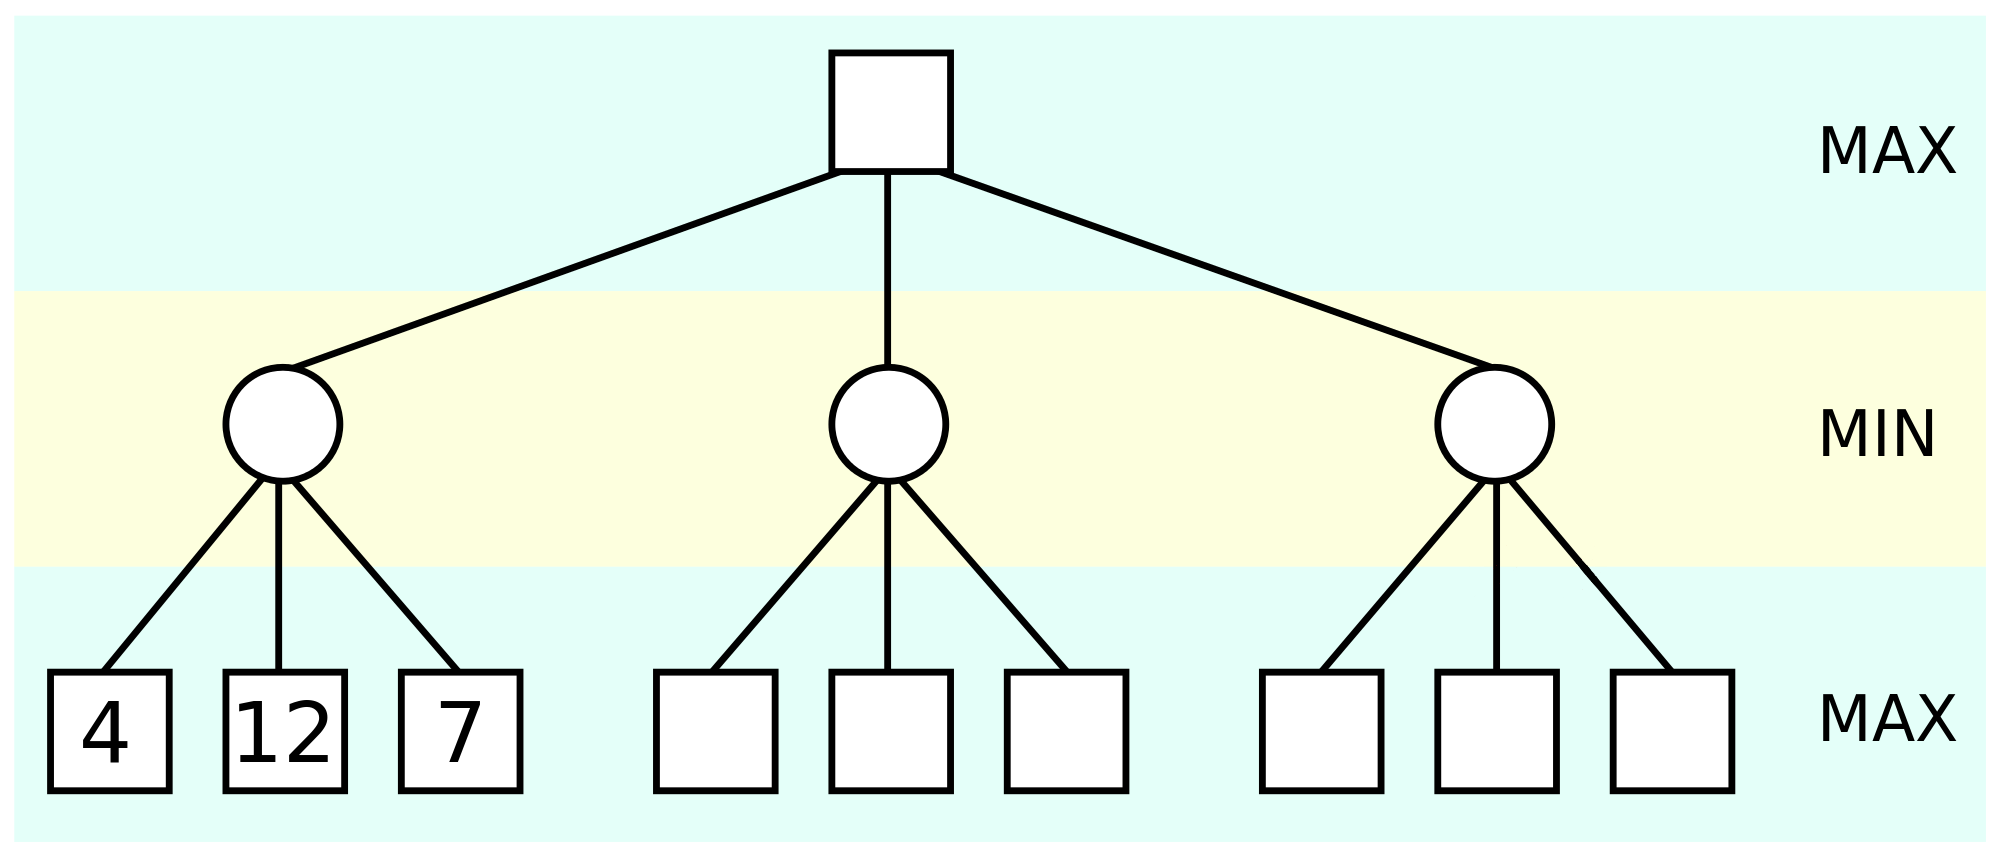
\includegraphics[width=\textwidth,height=\textheight,keepaspectratio]{minimax5.png}
\end{center}
\end{frame}

\begin{frame}{Search: Minimax Algorithm (Example)}
\begin{center}
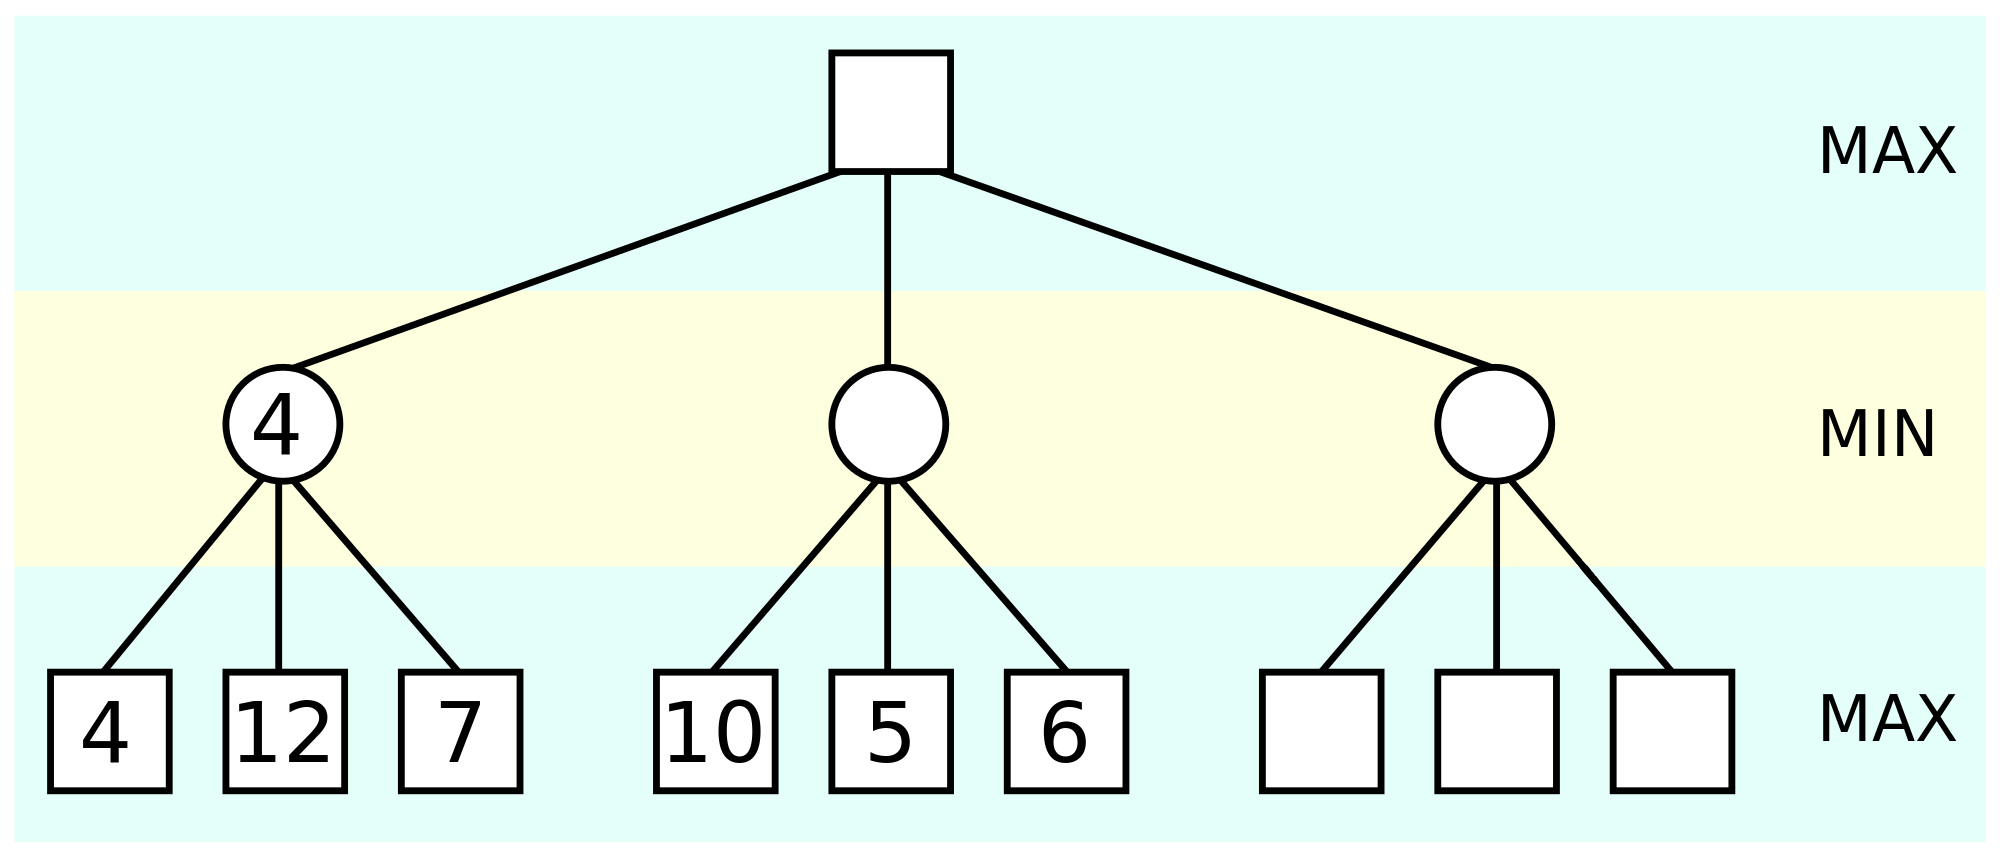
\includegraphics[width=\textwidth,height=\textheight,keepaspectratio]{minimax4.png}
\end{center}
\end{frame}

\begin{frame}{Search: Minimax Algorithm (Example)}
\begin{center}
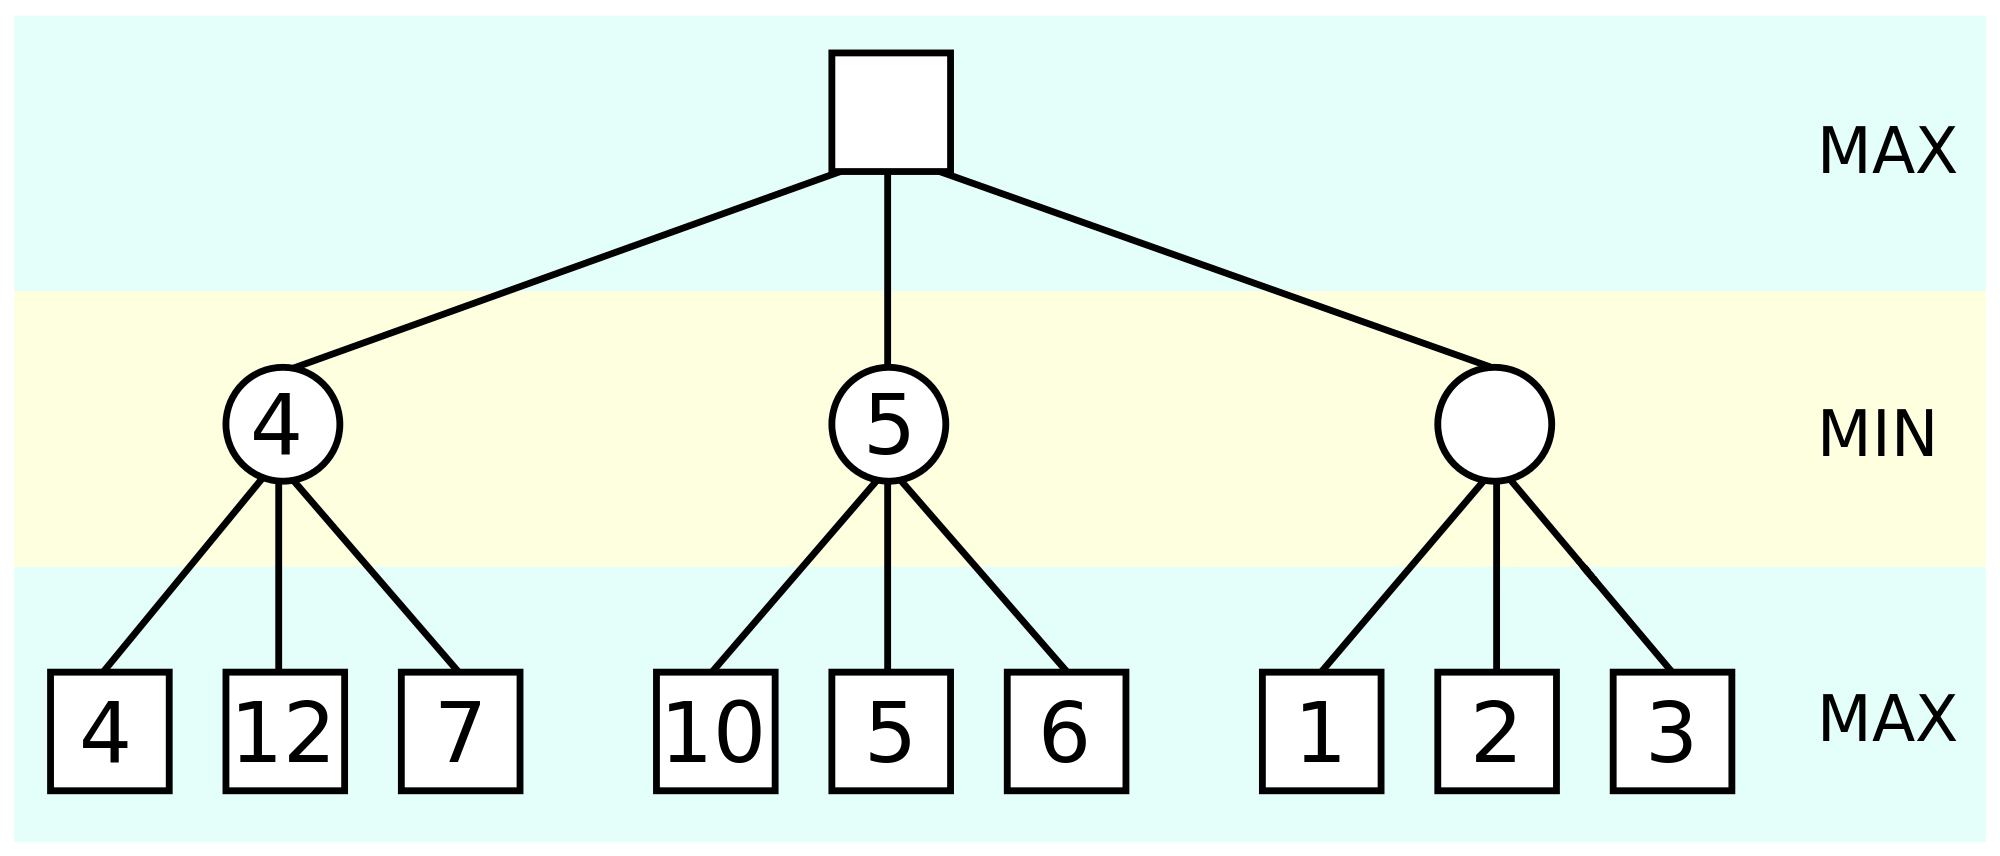
\includegraphics[width=\textwidth,height=\textheight,keepaspectratio]{minimax3.png}
\end{center}
\end{frame}

\begin{frame}{Search: Minimax Algorithm (Example)}
\begin{center}
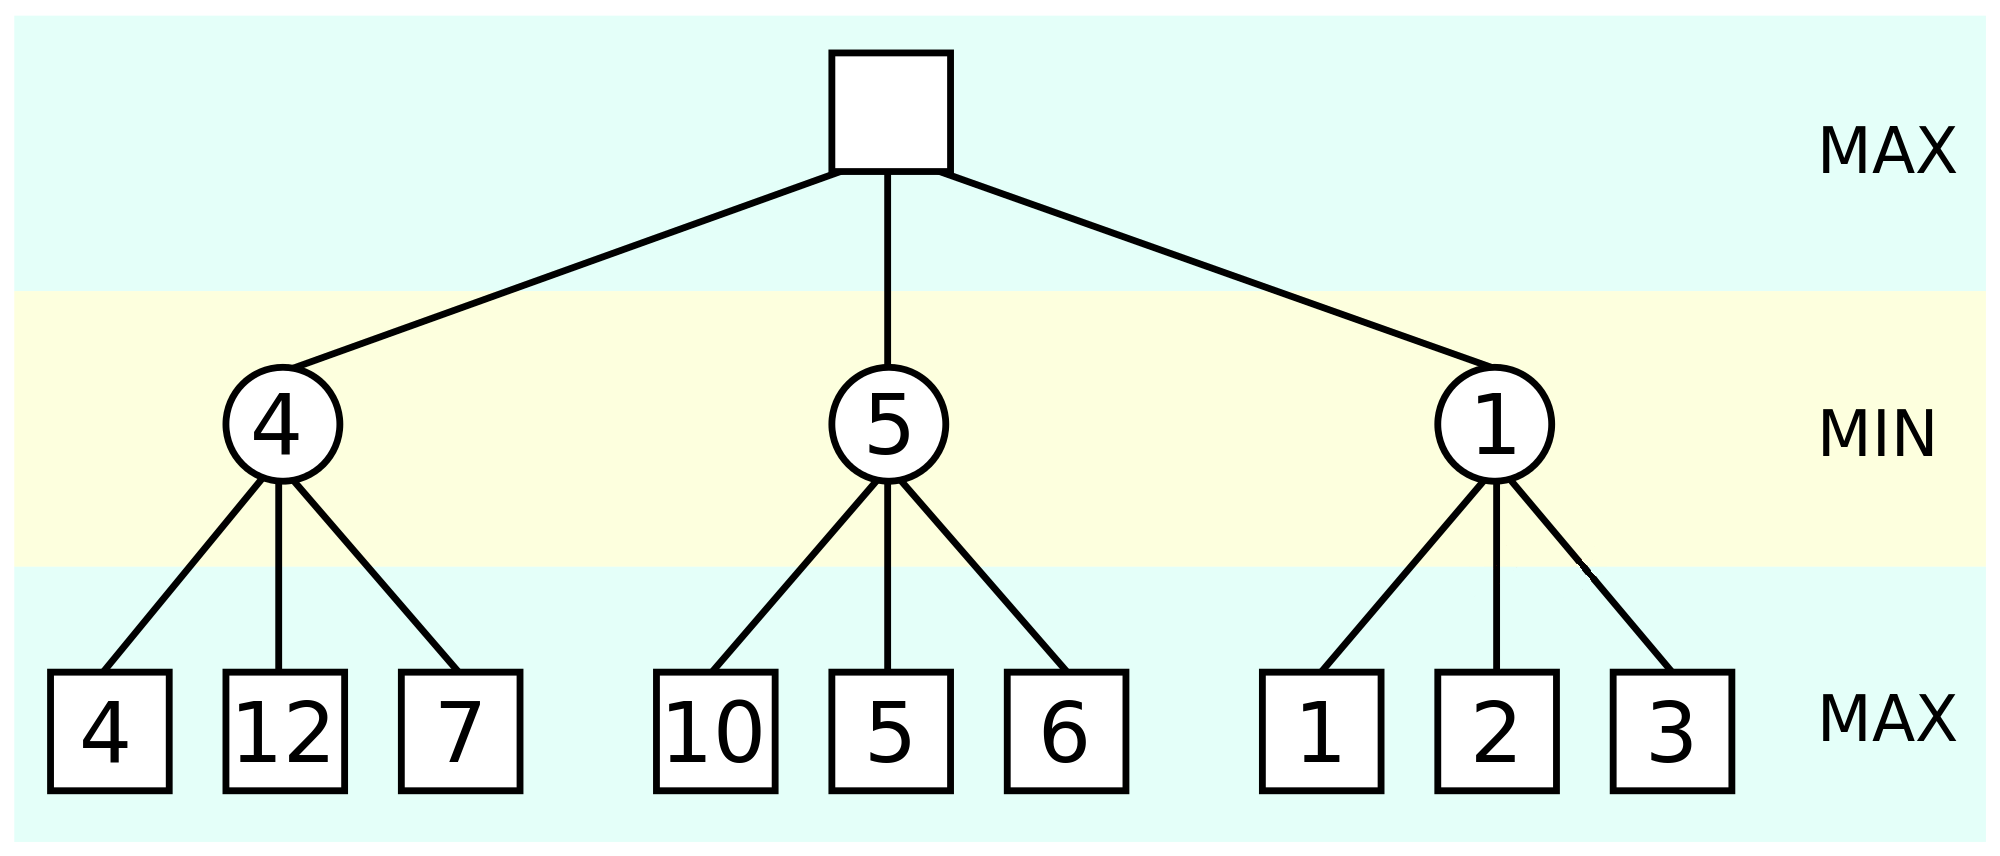
\includegraphics[width=\textwidth,height=\textheight,keepaspectratio]{minimax2.png}
\end{center}
\end{frame}

\begin{frame}{Search: Minimax Algorithm (Example)}
\begin{center}
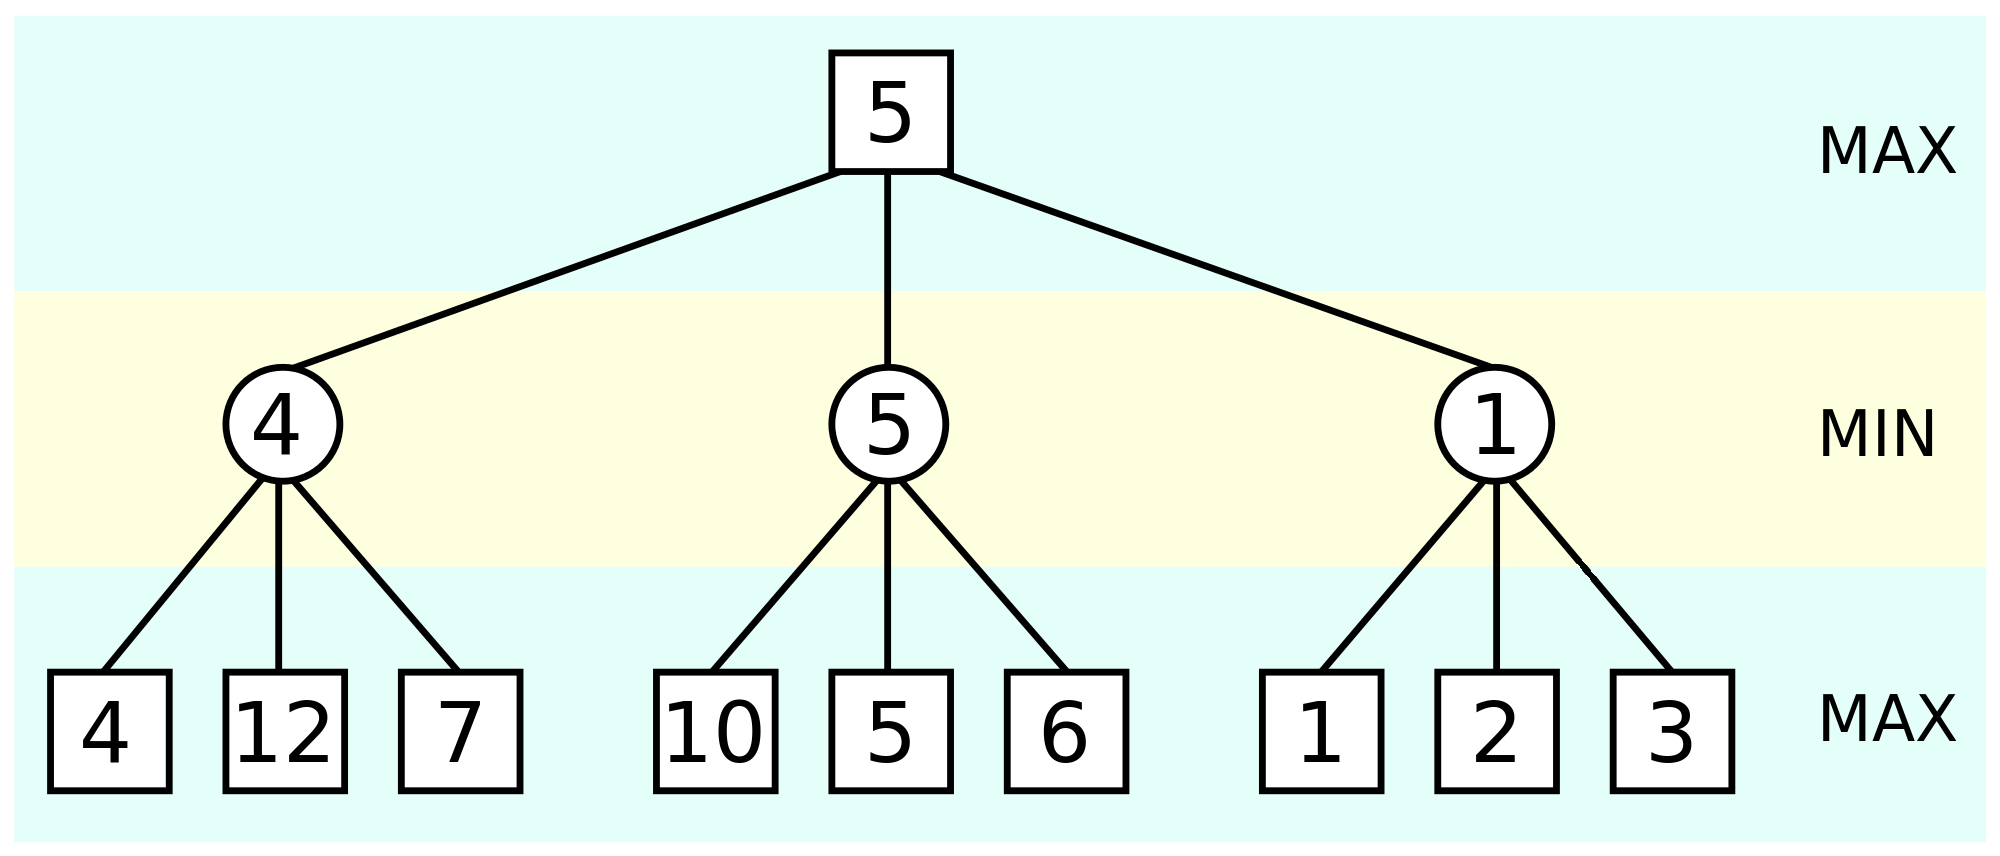
\includegraphics[width=\textwidth,height=\textheight,keepaspectratio]{minimax.png}
\end{center}
\end{frame}

\begin{frame}[fragile]{Search: Alpha-Beta Pruning}
\begin{itemize}
\item Problem with Minimax: too expensive
\item Prune the game tree by not considering irrelevant branches
\item Alpha $=$ Value of the best possible move you can make, that you have computed so far
\item Beta $=$ Value of the best possible move your opponent can make, that you have computed so far
\item If at any time Alpha $>=$ Beta, then your opponent can force a worse position than your best move so far, so there's no need to evaluate this move
\item Initially, start the search with Alpha $= -\infty$ and Beta $= \infty$
\end{itemize}
\end{frame}

\begin{frame}{Search: Alpha-Beta Pruning (Example)}
\begin{center}
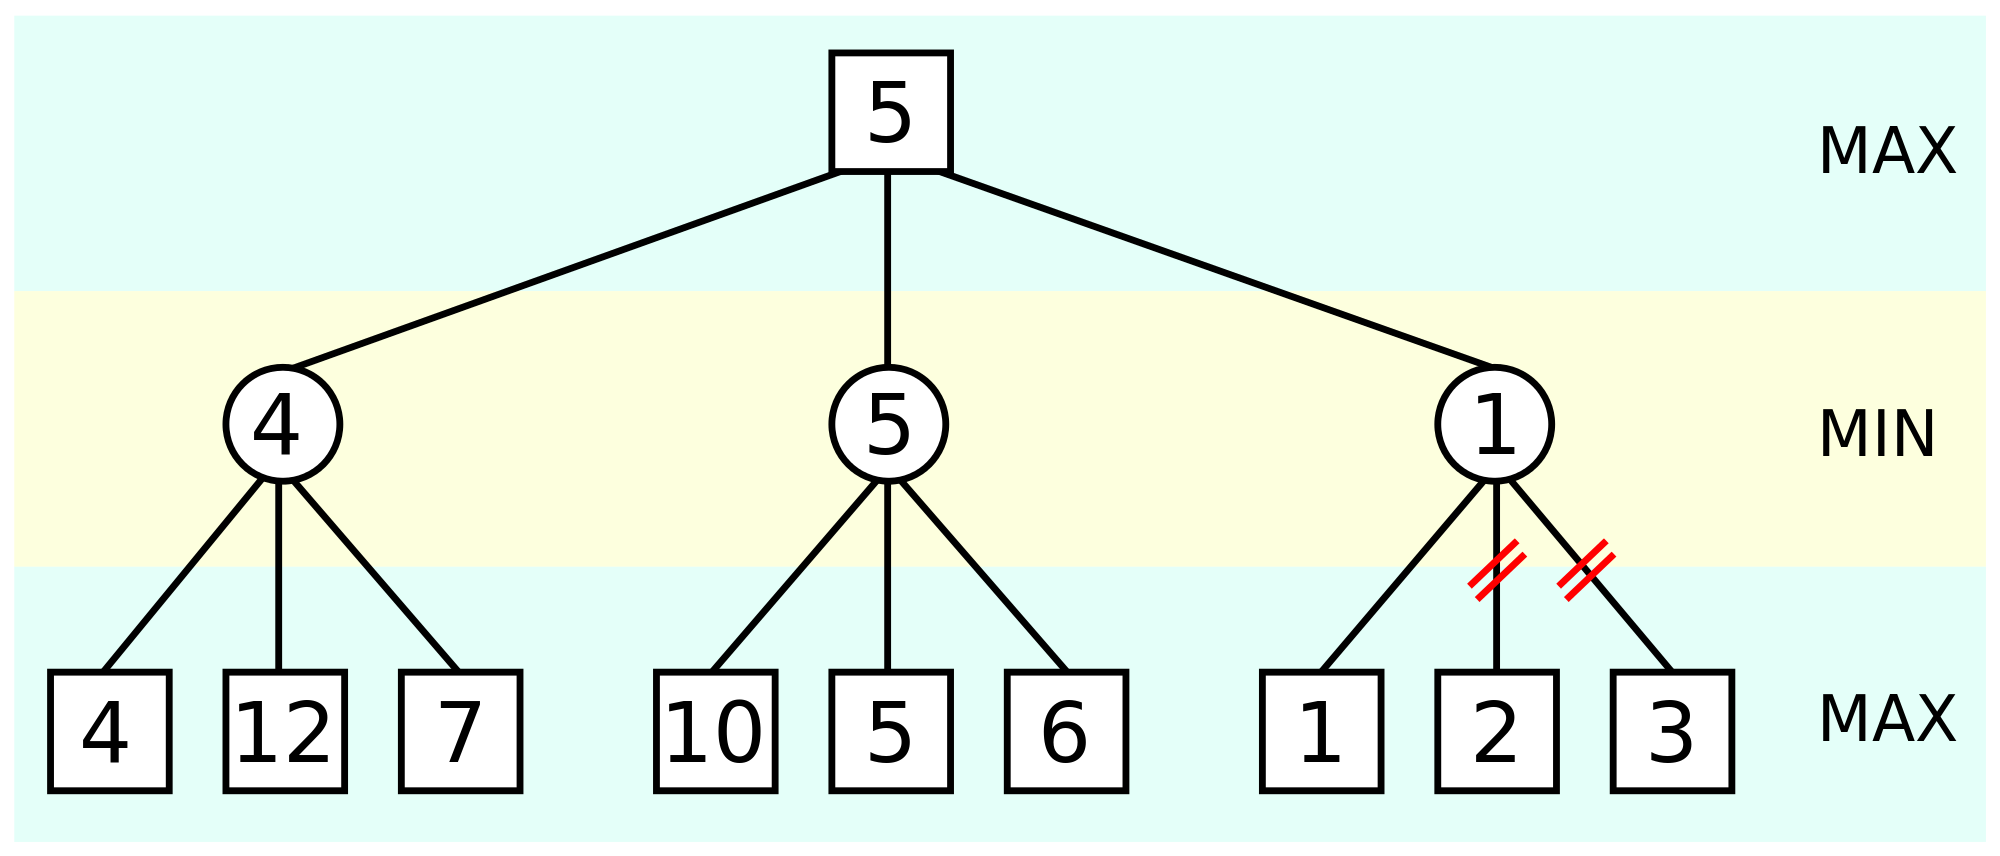
\includegraphics[width=\textwidth,height=\textheight,keepaspectratio]{AB_pruning2_svg.png}
\end{center}
\source{wikipedia.org}
\end{frame}

\begin{frame}{Search: Enchancements to Alpha-Beta Pruning}
\begin{itemize}
\item Move-ordering heuristics (e.g. killer moves) - search the best moves first to get an early cutoff for other moves
\item Quiescence search - don't stop searching the tree until a "quiet" position is reached
\item Iterative deepening - gradually increase the depth of the search tree
\item And many more (PVS, NegaScout, etc \dots)
\end{itemize}
\end{frame}

\begin{frame}{Search: Transposition Tables}
\begin{itemize}
\item What if we found a position which we've already searched before? (a transposition)
\item Rather than evaluate the position again, look up the evaluation from a table
\item Evaluations are indexed by a hash value
\item Hash value is generated (almost uniquely) by the position itself
\item E.g. Zobrist hashing
\end{itemize}
\end{frame}

%%%%%%%%%%%%%%%%%%%%%%%%%%%%%%%%%%%%%%%%%%%%%%%%%%%%%%%%%%%%%%%%%%%%%%%%%%%%%%%%%%%%%%%%%%
\section{Opening Books and Tablebases}

\begin{frame}{Opening Books}
\begin{itemize}
\item Chess openings are too complex
\item Often strategies prove to be good/bad after 20-30 moves
\item Choose the opening moves from a database of known Chess openings
\end{itemize}
\end{frame}

\begin{frame}{Endgame Tablebases}
\begin{itemize}
\item Endgames are surprisingly complex
\item Tablebases allow perfect play of the endgame
\item Unfeasible for large number of pieces
  \begin{itemize}
  \item[\textbullet] 4-piece tablebases $\sim 30$ Mb
  \item[\textbullet] 5-piece tablebases $\sim 7$ Gb
  \item[\textbullet] 6-piece tablebases $\sim 1.2$ Tb
  \item[\textbullet] 7-piece tablebases $\sim 140$k Tb!
  %% Aside: longest forced checkmate for 7 pieces is ~550 moves long
  \end{itemize}
\end{itemize}
\end{frame}

%%%%%%%%%%%%%%%%%%%%%%%%%%%%%%%%%%%%%%%%%%%%%%%%%%%%%%%%%%%%%%%%%%%%%%%%%%%%%%%%%%%%%%%%%%
\section{Recap and Conclusion}

\begin{frame}{Summary: Components of a Chess Engine}
\begin{itemize}
\item Board representation - How is a chess position stored?
\item Move generation - How do we generate all legal moves for a position quickly
\item Evaluation - How to assess a given position based on various factors
\item Search - How to find the best possible move in a tree of game positions
\item Opening books and Tablebases - Tools to help computers play the opening and endgame
\end{itemize}
\end{frame}

\begin{frame}{Future of Chess AI}
\begin{itemize}
\item We will probably never solve Chess ($\sim 10^{120}$ possible positions in a typical game)
\item Stockfish (open-source) and Komodo (closed-source, commercial) continue to improve
\item Diminishing returns for additional search
\item Can we make more "human-like" evaluation methods work (e.g. pattern recognition, general planning)?
\end{itemize}
\end{frame}

\begin{frame}{}
  \centering
  \vspace{50pt} 
  \LARGE
  \emph{Questions?}
  \small
  \vspace{30pt}
  \linebreak
  Chess Programming Wiki: \linebreak
  https://chessprogramming.wikispaces.com
\end{frame}

\end{document}

\section{Some \LaTeX{} Examples}

\subsection{Tables and Figures}

\begin{frame}{Tables and Figures}
\begin{itemize}
\item Use \texttt{tabular} for basic tables --- see Table~\ref{tab:widgets}, for example.
\item You can upload a figure (JPEG, PNG or PDF) using the files menu. 
\item To include it in your document, use the \texttt{includegraphics} command (see the comment below in the source code).
\end{itemize}
% Commands to include a figure:
%\begin{figure}
%\includegraphics[width=\textwidth]{your-figure's-file-name}
%\caption{\label{fig:your-figure}Caption goes here.}
%\end{figure}
\begin{table}
\centering
\begin{tabular}{l|r}
Item & Quantity \\\hline
Widgets & 42 \\
Gadgets & 13
\end{tabular}
\caption{\label{tab:widgets}An example table.}
\end{table}
\end{frame}

\subsection{Mathematics}

\begin{frame}{Readable Mathematics}
Let $X_1, X_2, \ldots, X_n$ be a sequence of independent and identically distributed random variables with $\text{E}[X_i] = \mu$ and $\text{Var}[X_i] = \sigma^2 < \infty$, and let
$$S_n = \frac{X_1 + X_2 + \cdots + X_n}{n}
      = \frac{1}{n}\sum_{i}^{n} X_i$$
denote their mean. Then as $n$ approaches infinity, the random variables $\sqrt{n}(S_n - \mu)$ converge in distribution to a normal $\mathcal{N}(0, \sigma^2)$.
\end{frame}


\begin{frame}
\frametitle{Famous Composers}
\begin{center}
\rowcolors{1}{RoyalBlue!20}{RoyalBlue!5}
\begin{tabular}{|l|c|}\hline
J.\ S.\ Bach & 1685--1750 \\
W.\ A.\ Mozart & 1756--1791 \\
L.\ Beethoven & 1770--1827 \\
F.\ Chopin & 1810--1849 \\
R.\ Schumann & 1810--1856 \\
B.\ Bartok & 1881--1945 \\ \hline
\end{tabular}
\end{center}
\end{frame}

\begin{frame}
\frametitle{Two Column Output}
\begin{columns}[c]
\column{1.5in}
Practical \TeX\ 2005\\
Practical \TeX\ 2005\\
Practical \TeX\ 2005
\column{1.5in}
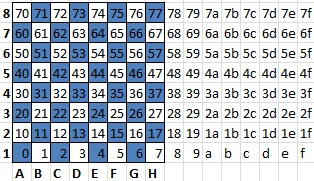
\includegraphics[width=\textwidth,keepaspectratio]{88board.jpg}
\end{columns}
\end{frame}


RESOURCES:

- Beamer tutorial
https://www.tug.org/pracjourn/2005-4/mertz/mertz.pdf

- History of AI in computer chess
http://hightechhistory.com/2011/04/21/a-history-of-computer-chess-%E2%80%93-from-the-mechanical-turk-to-%E2%80%9Cdeep-blue%E2%80%9D/

- Useful timeline of Computer Chess
http://www.thebestschools.org/magazine/brief-history-of-computer-chess/

- (old?) Chess AI Presentation
http://www.cs.bham.ac.uk/~jxb/IAI/w9g.pdf

- How computers play chess
http://www.slideshare.net/carlosjustiniano2/how-computers-play-chess-26552933

- Paper on how Stockfish works
http://rin.io/chess-engine/

- MiniMax Algorithm
http://web.cs.wpi.edu/~rich/courses/imgd4000-d09/lectures/E-MiniMax.pdf

- Diminishing returns on additional search
https://chessprogramming.wikispaces.com/Depth?responseToken=b08a10614bc08c7eb5cf32c8497f34e8#cite_note-7

- Cool Alpha-Beta pruning applet
http://will.thimbleby.net/algorithms/doku.php?id=minimax_search_with_alpha-beta_pruning

- Alpha-Beta pruning and minimax
http://web.cecs.pdx.edu/~mm/AIFall2011/GamePlaying.pdf

CODE EXAMPLES:
\begin{frame}{What is Chess?}
\vskip 1cm
\begin{block}{Examples}
Some examples of commonly used commands and features are included, to help you get started.
\end{block}
\end{frame}
